%%%%%%%%%%%%%%%%%%%%%%%%%%% asme2e.tex %%%%%%%%%%%%%%%%%%%%%%%%%%%%%%%
% Template for producing ASME-format articles using LaTeX            %
% Written by   Harry H. Cheng                                        %
%              Integration Engineering Laboratory                    %
%              Department of Mechanical and Aeronautical Engineering %
%              University of California                              %
%              Davis, CA 95616                                       %
%              Tel: (530) 752-5020 (office)                          %
%                   (530) 752-1028 (lab)                             %
%              Fax: (530) 752-4158                                   %
%              Email: hhcheng@ucdavis.edu                            %
%              WWW:   http://iel.ucdavis.edu/people/cheng.html       %
%              May 7, 1994                                           %
% Modified: February 16, 2001 by Harry H. Cheng                      %
% Modified: January  01, 2003 by Geoffrey R. Shiflett                %
% Use at your own risk, send complaints to /dev/null                 %
%%%%%%%%%%%%%%%%%%%%%%%%%%%%%%%%%%%%%%%%%%%%%%%%%%%%%%%%%%%%%%%%%%%%%%

%%% use twocolumn and 10pt options with the asme2e format
\documentclass[twocolumn,10pt]{asme2e}
\special{papersize=8.5in,11in}
\usepackage{amsmath}
\usepackage{amssymb}
\usepackage{graphicx}
\usepackage{multirow}


%% The class has several options
%  onecolumn/twocolumn - format for one or two columns per page
%  10pt/11pt/12pt - use 10, 11, or 12 point font
%  oneside/twoside - format for oneside/twosided printing
%  final/draft - format for final/draft copy
%  cleanfoot - take out copyright info in footer leave page number
%  cleanhead - take out the conference banner on the title page
%  titlepage/notitlepage - put in titlepage or leave out titlepage
%  
%% The default is oneside, onecolumn, 10pt, final

%%% Replace here with information related to your conference
\confshortname{MSEC2022}
\conffullname{the ASME 2022 International Manufacturing Science Engineering \&\\
              Engineering Conference}

%%%%% for date in a single month, use
%\confdate{24-28}
%\confmonth{September}
%%%%% for date across two months, use
\confdate{June 27 - July 1}
\confyear{2022}
\confcity{West Lafayette, Indiana}
\confcountry{USA}

%%% Replace DETC2009/MESA-12345 with the number supplied to you 
%%% by ASME for your paper.
\papernum{MSEC2022-85981}

%%% You need to remove 'DRAFT: ' in the title for the final submitted version.
\title{iStructure: An Open Source structural design framework}
%%% for the discussion section only
%\usepackage{helvet}
%\title{\fontfamily{phv}\selectfont{\Huge{DRAFT: AN ARTICLE CREATED USING \LaTeX2\raisebox{-.3ex}{$\epsilon$}\ IN ASME FORMAT}}}

%%% first author
\author{Juan D. Arg\"uello
    \affiliation{
    GIEMA\\
    Escuela de Ingenier\'ia Mec\'anica\\
	Universidad Industrial de Santander\\
	Bucaramanga, Colombia\\
	Email: juan2198189@correo.uis.edu.co
    }	
}

%%% second author
%%% remove the following entry for single author papers
%%% add more entries for additional authors
\author{Octavio A. Gonz\'alez
    \affiliation{
    GIEMA\\
    Escuela de Ingenier\'ia Mec\'anica\\
	Universidad Industrial de Santander\\
	Bucaramanga, Colombia\\
	Email: agonzalez@uis.edu.co
    }	
}

\begin{document}

\maketitle    

%%%%%%%%%%%%%%%%%%%%%%%%%%%%%%%%%%%%%%%%%%%%%%%%%%%%%%%%%%%%%%%%%%%%%%
\begin{abstract}
{\it Artificial Intelligence (AI) can be defined as a developed technology which has come to supplant cyclic tasks in different work environments. It allows the optimization of operational costs and productivity.  One of the most affected, and challenging, industries around the world  is  the  civil  industry, principally at the design stage. To optimize the process of design, structural and cost analysis, we created the iStructure project, which is a manufacturing tool that automate the design of structural members. It is a python-based framework library that, in its first version, can automate the design procedure of Mezzanine Floor Racking Systems. It allows the user to: specify the cross-section geometries of the structural members and predicts its geometric properties by the Finite Element Method – FEM; define the modular area distribution per floor; select the minimum cost cross-sections of the structural members which can resist the specified load conditions; create an automatic report, in LaTeX/PDF, which illustrates the design procedure (according to ANSI MH16.1, AISI S100 and ASCE 7-16 North American standards) and the costs of the structure; and elaborates automatic 3D CAD plans in DXF format.  }
\end{abstract}

\section*{INTRODUCTION}

Automation in engineering is widely applied to save both time and money. The construction industry is falling behind others in terms of making productivity gains \cite{CHEN201822}. It can be concluded that technology adoption in the construction industry is accelerating at a slower pace when compared to industries like finance, entertainment and education, among others \cite{AKINOSHO2020101827}.  Various reasons have been invoked to explain negative productivity trends, such as shifts within construction, increases in land-use regulation and the use of questionable deflators\cite{LEE2021103680}. Productivity in the construction industry is unstable or sometimes on the decline with under-investment in technology being a partial culprit \cite{unknown}. According to UKGOV \cite{hm2013construction}, digitisation will allow construction sector to deliver cheaper, faster and smarter services with low-cost labour. Even manufacturing process would be optimized thanks to these multiple advantages.

When talking about automation, people could have different interpretations of what construction automation means. For example, most designers consider it as a way to automate the planning and design of projects, but construction contractors consider it as the use of robots for onsite tasks \cite{CHEN201822}. Over the decades, the necessity of implementing technology in the construction industry has been emphasized in multiple studies because of the aging workforce and the increasing complexity of constructions. Although a large number of researches have been conducted and various types of systems and technologies have been developed, the field is far from mature \cite{CAI2019100989, BOCK2015113}. 

Unlike concrete buildings and bridges, metallic structures does not require special architectural design because its purpose is basically to increase the storage area of goods and raw materials of different industries in warehouses \cite{YIN201972, 10.22260/ISARC2000/0031}. Thanks to it, there is an innovation opportunity in the automation of the design stage of metallic structures. The present work focus on Mezzanine Floor Racking Systems and in the explanation of the logic behind a structural design framework, made by the authors, in Python - Jupyter, which starts by asking the user the area of the structure and load conditions. Then, it selects the structural members (beams, columns, and joists), evaluated by the FEM and selected by a defined design procedure, based on AISI S-100-16 \cite{S100}, ANSI MH16.1 \cite{MH16.1} and ASCE 7-16 \cite{ASCE} North American standards. Finally, the results are an economic report, an engineering design report and the CAD draws, 2D and 3D, of the structure.

%%%%%%%%%%%%%%%%%%%%%%%%%%%%%%%%%%%%%%%%%%%%%%%%%%%%%%%%%%%%%%%%%%%%%%
\section*{DESIGN METHODOLOGY}

Mezzanine Floor Racking Systems are modular structures which consist of beams, columns and joists. The resistance of a structural member rely on the material, geometry of the section and the length of the member. By default, if not specified, the framework is programmed to work with steel ASTM A1011 SS Grade 36/2. Other materials can be defined and selected by the user. Even composite materials can be implemented.

The user should define the cross sections database for every structural member: beam, column and joist. To predict the cross section properties, iStructure implements the \textit{section properties} Open Source library \cite{sectionproperties}, so the user only has to specify cross sections geometry and classify them depending on the kind of structural member. Geometric, plastic and warping analysis is developed by a Finite Element Method simulation of the cross section. 

Having the cross sections database established, the next step is to define the dimensions of the structure and load conditions per floor. With this information, the user can specify the framework to evaluate the area of the structure and list the cross sections that resist load conditions according to ANSI MH16.1, AISI S100 and ASCE 7-16 North American standards. If the framework is not able to find any cross section in the database that supports load conditions, it will notify the user and give suggestions on how to redesign the area of floors to meet design criteria. 

Once the cross sections are selected, the user can ask the framework for automatic engineering reports, made in LaTeX/PDF, and CAD draws of the final structure.

%%%%%%%%%%%%%%%%%%%%%%%%%%%%%%%%%%%%%%%%%%%%%%%%%%%%%%%%%%%%%%%%%%%%%%

\subsection*{STRUCTURAL DESIGN PROCEDURE}

The geometrical and wrap properties of the cross sections are calculated by the Finite Element Method. For the 2D linear elasticity problem, the unknown displacement field $u$, taking values in $\Omega \subset \mathbb{R} ^2$, is the solution of the boundary value problem, given by:

\begin{equation}
- \nabla \cdot \sigma (u) = b \quad \quad \quad \quad  \text{in } \Omega
\end{equation}

\begin{equation}
\sigma (u) \cdot n = t \quad \quad \quad \quad \quad  \text{on } \Gamma _N
\end{equation}

\begin{equation}
u = 0 \quad \quad \quad \quad \quad \quad \quad \text{on } \Gamma _D
\end{equation}


Where $\Gamma _N$ and $\Gamma _D$ denote the Neumann and Dirichlet boundaries with $\partial \Omega = \Gamma _N \cup \Gamma _D$  and $\Gamma _N \cap \Gamma _D = \emptyset$. The Dirichlet boundary condition in Eqn 3 is assumed to be homogeneous. The weak form of the problem reads: Find $u \in V$ sucha that

\begin{equation}
\forall v \in V \quad \quad \quad a (u,v) = l(v)
\end{equation}

where V is the standard test space for the elasticity problem such that $V = {v | v }$, and 

\begin{equation}
	a (u,v) = \int _\Omega \epsilon (u ) ^T D \epsilon (v) d \Omega = \int _\Omega \sigma (u)^T D ^{-1} \sigma (v) d\Omega
\end{equation}

\begin{equation}
l (v) := \int _\Omega b^T v d\Omega + \int _{\Gamma _N} t^T v d \Gamma
\end{equation}

where $D$ is the elasticity matrix of the constitutive relation $\sigma = D \epsilon$, $\sigma$ and $\epsilon$ denote the stress and strain operators.

Let $u ^h$ be a finite element approximation to $u$. The solution lies in a functional space $V ^h \subset V$ associated with a mesh of isoparametric finite elements of characteristic size h, which is defined by equation (3). 

Using a variational formulation of the problem, Eqns 1-3, and a finite element approximation $u^h = N u^{e}$, where $N$ denotes the shape functions of order $p$, we obtain a system of linear equations to solve the displacements at nodes $u^e$:

\begin{equation}
K U = f
\end{equation}

where $K$ is the stiffness matrix, $U$ is the vector of nodal displacements and $f$ is the load vector.

Defined the cross sections properties, the area of the structure and the distributed load per area, we define the dead load, live load and product load the structure will have to resist. 

\begin{equation}
	D = W_t L 
	\label{dead}
\end{equation}

From Equation \ref{dead}, $D$ represents the dead load, $W_t$ is the weight per length and $L$ is the length of the member.

\begin{equation}
L = k_w T_A
\label{live}
\end{equation}

Where $L$ is the live load, $k_w$ is the kind of weight the structure has to resist and $T_A$ is the tributary area of the structural member. According to ASCE/SEI7, the kind of weight could be a \textit{"light weight"} $\left(6 kN / m^2 \right)$ or a \textit{"heavy weight"} $\left(11.97 kN / m^2 \right)$.

\begin{equation}
P = W_A T_A
\label{product}
\end{equation}

From equation \ref{product}, $P$ is the product load and $W_A$ is the weight of the area (given by the user).

According to ANSI MH16.1 and ASCE/SEI7-16, the equivalent distributed load of the structural member is defined by Equation \ref{eqDistLoad}.

\begin{equation}
w = \frac{1.2 D + 1.4 P + 1.6 L}{l}
\label{eqDistLoad}
\end{equation}

From Eq. \ref{eqDistLoad}, $l$ is the length of the structural member. 

The structural design of members in compression is defined on Chapter E in AISI S100-16 standard. It dictates that "the nominal axial strength $P_{ne}$ for yielding, and global buckling shall be calculated with a safety factor and a resistance factor to determine available axial strength $\left( \phi _c P_{ne} \right)$".

\begin{equation}
	P_{ne} = A_g F_n \\
	\phi _c = 0.85
\end{equation}

Where $A_g$ is the gross area, $F_n$ is the compressive stress, which shall be calculated as follows.

\begin{equation}
	F_n = \left( 0.658 ^{\lambda _c ^2} \right) F_y \quad \quad \lambda _c \leq 1.5
\end{equation}

\begin{equation}
	F_n = \frac{0.877}{\lambda _c ^2}  F_y  \quad \quad \lambda _c > 1.5
\end{equation}

Where 

\begin{equation}
	\lambda _c = \sqrt{\frac{F_y}{F_{cre}}}
	\label{lambda}
\end{equation}

From Eq. \ref{lambda}, $F_{cre}$ correspond to the least of the applicable elastic global buckling stress and $F_y$ to the yield stress. The flexural buckling stress can be calculated as follows.

\begin{equation}
	F_{cre} = \frac{1}{2 \beta} \left[(\sigma _{ex} + \sigma _t ) - \sqrt{(\sigma _{ex} + \sigma _t)^2 - 4 \beta \sigma _{ex} \sigma _t} \right]
\end{equation}

Where 

\begin{equation}
\beta = 1 - (x_o/r_o)^2
\label{beta}
\end{equation}

From Eq. \ref{beta}, $x_o$ is the distance from centroid to shear center in principal x-axis direction and $r_o$ is the polar radius of gyration of the cross-section about shear center which is given by Eq. \ref{ro}.

\begin{equation}
r_o = \sqrt{r_x ^2 + r_y ^2 + x_o ^2}
\label{ro}
\end{equation}

For compression members, shear stress is given by Eq. \ref{compShear}.

\begin{equation}
\sigma _t =  \frac{1}{A r_o ^2} \left[G J + \frac{\pi ^2 E C_w}{(K_t L_t)^2} \right]
\label{compShear}
\end{equation}

Where $A$ is the full unreduced cross-sectional area of member, $G$ is the shear modulus, $J$ is the Saint-Venant torsion constant of the section, $E$ is the modulus of elasticity, $C_w$ is the torsional warping constant, $K_t$ is the effective length factor and $L_t$ is the unbraced length of the member.

\begin{equation}
\sigma _{ex} = \frac{\pi ^2 E}{(K_x L_x / r_x)^2}
\label{exComp}
\end{equation}

From Eq. \ref{exComp}, $K_x$ is the effective length factor for bending about x-axis and $L_x$ is the unbraced length of the member around x-axis.

The elastic buckling stress for singly- or doubly- symmetric sections bending about the symmetric axis shall be calculated as follows \cite{ASCE}.

\begin{equation}
	F_{cre} = \frac{C_b r_o A}{S_f} \sqrt{\sigma _{ey} \sigma _t}
\end{equation}

Where

\begin{equation}
C_b = \frac{12.5 M_{max}}{2.5 M_{max} + 3 M_A + 4 M_B + 3 M_C}
\label{Cb}
\end{equation}

From Eq. \ref{Cb}, $M_{max}$ is the absolute value of maximum moment, $M_A$ is the absolute value of moment at quarter point, $M_B$ is the absolute value of moment at centerline and $M_C$ is the absolute value of moment at three-quarter point.

\begin{equation}
\sigma _{ey} = \frac{\pi ^2 E}{(K_y L_y / r_y)^2}
\label{sigma_ey}
\end{equation}



%%%%%%%%%%%%%%%%%%%%%%%%%%%%%%%%%%%%%%%%%%%%%%%%%%%%%%%%%%%%%%%%%%%%%%
\section*{RESULTS}

As a result of this work, we will give an example of how to develop a structural design of a Mezzanine structure with the iStructure framework. We will use the default material specified by the framework, which is steel ASTM A1011 SS Grade 36/2. The properties of this material can be appreciated on Table \ref{steel}.

\begin{table}[t]
\centering
\caption{STRENGTH PROPERTIES.}
\begin{tabular}{c c}
 & \\
\hline
\textbf{Parameter} & \textbf{Value} \\ \hline
Density $\left[kg/m^3\right]$ & 7850 \\ \hline
Young Modulus $[GPa]$ & 200 \\ \hline
Coefficient of Poisson & 0.3 \\ \hline
Yield strength $[MPa]$ & 248.25 \\ \hline
Ultimate strength $[MPa]$ & 440 \\ \hline
\end{tabular}
\label{steel}
\end{table}

We will evaluate the suggested cross sections shown on Fig. \ref{sections}.

\begin{figure}[t]
\centering
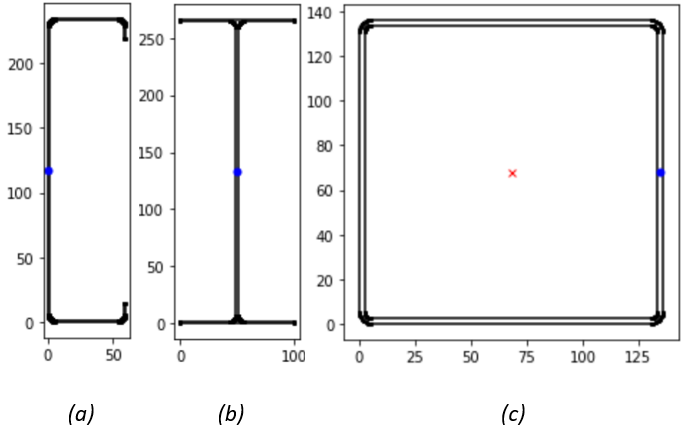
\includegraphics[width=9cm]{Images/sections.PNG}
\caption{CROSS SECTIONS. (a) JOIST SECTION, (b) BEAM SECTION AND (c) COLUMN SECTION.}
\label{sections}
\end{figure}

Evaluating its properties with a tetrahedral mesh of $3 [mm]$, partial results can be seen on Table \ref{properties}.

\begin{table}[t]
\centering
\caption{CROSS SECTION PROPERTIES}
\vspace{0.5cm}
\begin{tabular}{c | c c c}
\hline
\multirow{2}{*}{\textbf{Parameter}} & & \textbf{Section} \\  \cline{2-4}
 & Joist & Beam & Column \\ \hline
$A [mm^2]$ & $554.7$  & $979.1$  & $1316.6$  \\ \hline
$I_{xx} [mm^4]$ & $4283927$ & $9404210$ & $3883078$ \\ \hline
$I_{xy} [mm^4]$ & $-1.5*10^{9}$ & $-1.3*10^{8}$ & $6.5 * 10^{9}$ \\ \hline
$I_{yy} [mm^4]$ & $229625$ & $250483$ & $3883078$ \\ \hline
$r_x [mm]$ & $87.9$ & $98.0$ & $54.3$ \\ \hline
$r_y [mm]$ & $20.3$ & $16.0$ & $54.3$ \\ \hline
$J [mm^4]$ & $414.7$ & $1822.5$ & $6027803$ \\ \hline
\end{tabular}
\label{properties}
\end{table}

For this example, we will evaluate load distribution over the area shown on Fig. \ref{DistArea}, where orange lines correspond to joists and blue lines to the beams of the structure. Joist separation is constant and equal to $0.5 [m]$. The distributed load that is expected the structure to resist is of $500 [kg / m^2]$.

\begin{figure}[t]
\centering
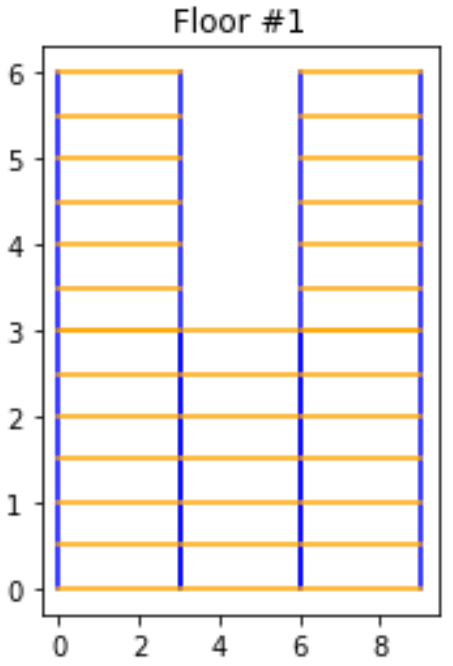
\includegraphics[width=0.2\textwidth]{Images/area.PNG}
\caption{AREA OF THE STRUCTURE.}
\label{DistArea}
\end{figure} 

The loads summary can be appreciated on Table \ref{loads}, as well as the results of the structural design procedure defined on Eqs (\ref{dead} - \ref{sigma_ey}).

\begin{table}[t]
\centering
\caption{SUMMARY OF RESULTS}
\vspace{0.5cm}
\begin{tabular}{c | c c c}
\hline
\multirow{2}{*}{\textbf{Parameter}} & & \textbf{Section} \\  \cline{2-4}
 & Joist & Beam & Column \\ \hline
$D [kg]$  & $21.4$ & $125.7$ & $161.3$ \\ \hline
$L [kg]$ & $275.3$ & $275.3$ & $275.3$ \\ \hline
$P [kg]$ & $750.3$ & $6086.4$ & $6050.8$ \\ \hline
$w [kN/m]$ & $5.0$ & $29.8$ & $108.0$ \\ \hline
$M_u [kN \, m]$ & $5.4$ & $32.4$ & $121.5$ \\ \hline
$V_u [kN]$ & $7.3$ & $43.2$ & $162.0$ \\ \hline
$\sigma _{ex} [MPa]$ & $1726.7$ & $3258.5$ & $376.9$ \\ \hline
$\sigma _{ey} [MPa]$ & $113.0$ & $2325.0$ & $364.9$ \\ \hline
$\sigma _{t} [MPa]$ & $123.8$ & $3312.0$ & $56522.0$ \\ \hline
$M _{n} [kN \, m]$ & $6.5$ & $37.9$ & - \\ \hline
$P_{n} [kN]$ & - & - & $232.5$ \\ \hline

\end{tabular}
\label{loads}
\end{table}

It is also possible to corroborate the given results with FEM simulation results over the cross sections. For example, joist section behaviour can be appreciated on Fig. \ref{stress}.

\begin{figure}[t]
\centering
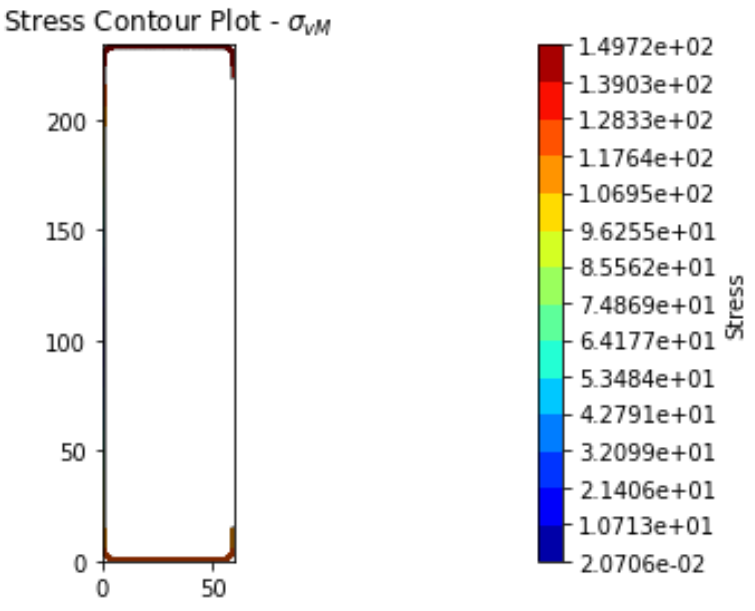
\includegraphics[width=8cm]{Images/vmJoist.PNG}
\caption{STRESS DISTRIBUTION OVER A JOIST SECTION.}
\label{stress}
\end{figure} 

Once the structural members have been selected, it is possible to elaborate automatic reports and CAD drawings. For example, the 3D CAD draw of the structure can be appreciated on Fig. \ref{CAD}.

\begin{figure}[t]
\centering
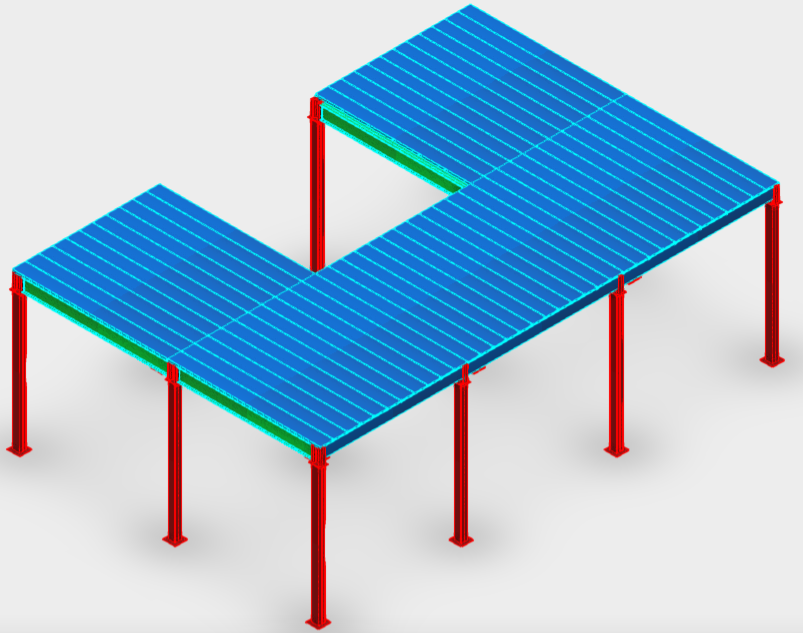
\includegraphics[width=8cm]{Images/RES.PNG}
\caption{3D CAD DRAWING OF THE DESIGNED STRUCTURE.}
\label{CAD}
\end{figure} 

%%%%%%%%%%%%%%%%%%%%%%%%%%%%%%%%%%%%%%%%%%%%%%%%%%%%%%%%%%%%%%%%%%%%%%
\section*{CONCLUSIONS}

iStructure is a framework that simplifies the structural design procedure. Its results gives confidence to the user because it can be validated with both North American standards and Finite Element Method analysis. Given the results shown on Fig. \ref{stress} and Table \ref{loads}, it is clear that the selected members can resist the defined load distribution. 

It is a fact that Mezzanine Floor Racking Systems are structures which fulfil storage of goods, and that it does not require any special architectural design. Despite of this, future investigations could propose different algorithms and methodologies that automate architectural design according to user needs.


%%%%%%%%%%%%%%%%%%%%%%%%%%%%%%%%%%%%%%%%%%%%%%%%%%%%%%%%%%%%%%%%%%%%%%
\begin{acknowledgment}

Thanks to Universidad Industrial de Santander and GIEMA for supporting this investigation.  

\end{acknowledgment}

%
\bibliographystyle{plain}
\bibliography{refs}



\end{document}
